\section{Experiments}

\subsection{Cover Traffic}

\begin{figure}
\begin{center}
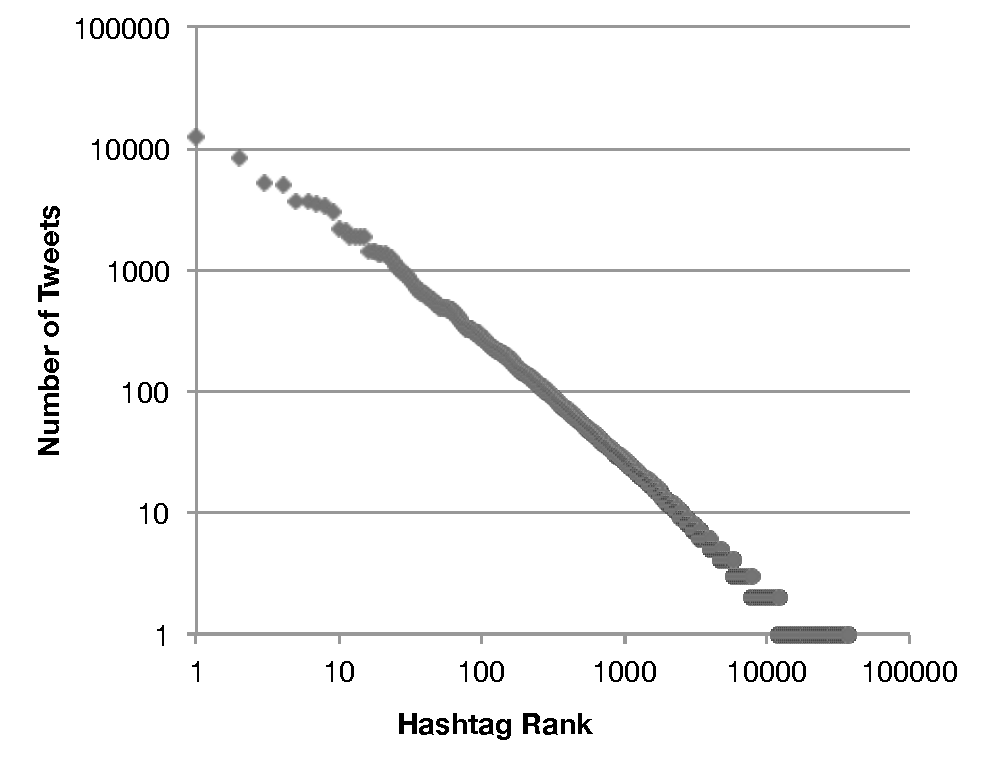
\includegraphics[scale=.5, viewport= 0cm 0cm 16.6cm 12.9cm]{hash-tag-dist.pdf}
\caption{2009 Twitter Hash Tag distribution on a log-log scale.
\label{fig:hash-dist}
}
\end{center}
\end{figure}

The power log scale shows us that there is a large spectrum of subscriber anonymity that can be taken advantage of. Colliding with popular tags gives you plausible deniability as there are relatively few tags dominating the space at a given time, and thus appear as legitimate interests. If there were a more even distribution of tags, then someone observing you following a particular tag would have less incentive to ignore suspicion that your activities might be objectionable to them. \hl{can we get a statistic on what the average number of tags someone follows is?}


\subsection{Collider}

In order to explore the feasibility of steering a particular Plain Tag to collide with an existing Short Tag, we built a collider tool. The tool takes in a Short Tag substring, \textit{T}, a prefix string, \textit{S}, a suffix length, \textit{L}, an alphabet 
\textit{A}. The collider finds the concatenations of \textit{S} and strings of length \textit{L} from \textit{A*} such that the truncated hash of the resultant string matches \textit{T}.

It has two modes of operation. In the default mode, he user specifies some number of tags to return that collide. The collider begins its scan at a random point in the search space and continues scanning until the requested number of tags are found. The second mode scans the entire search space, and therefore returns all matching tags for a given prefix and suffix length.

The search space, then, is of size $|A|^L$. If we wanted to match byte strings, $|A| = 256$, however, we decided to restrict the alphabet to alphanumeric characters due to Twitter's understanding of characters and not bytes, yielding $|A| = 62$. Additionally, the search space can be explored in parallel, giving the Collider executing on a system with \textit{P} processing units, a runtime of $O(\frac{62^L}{P})$.


\begin{figure}
\begin{center}
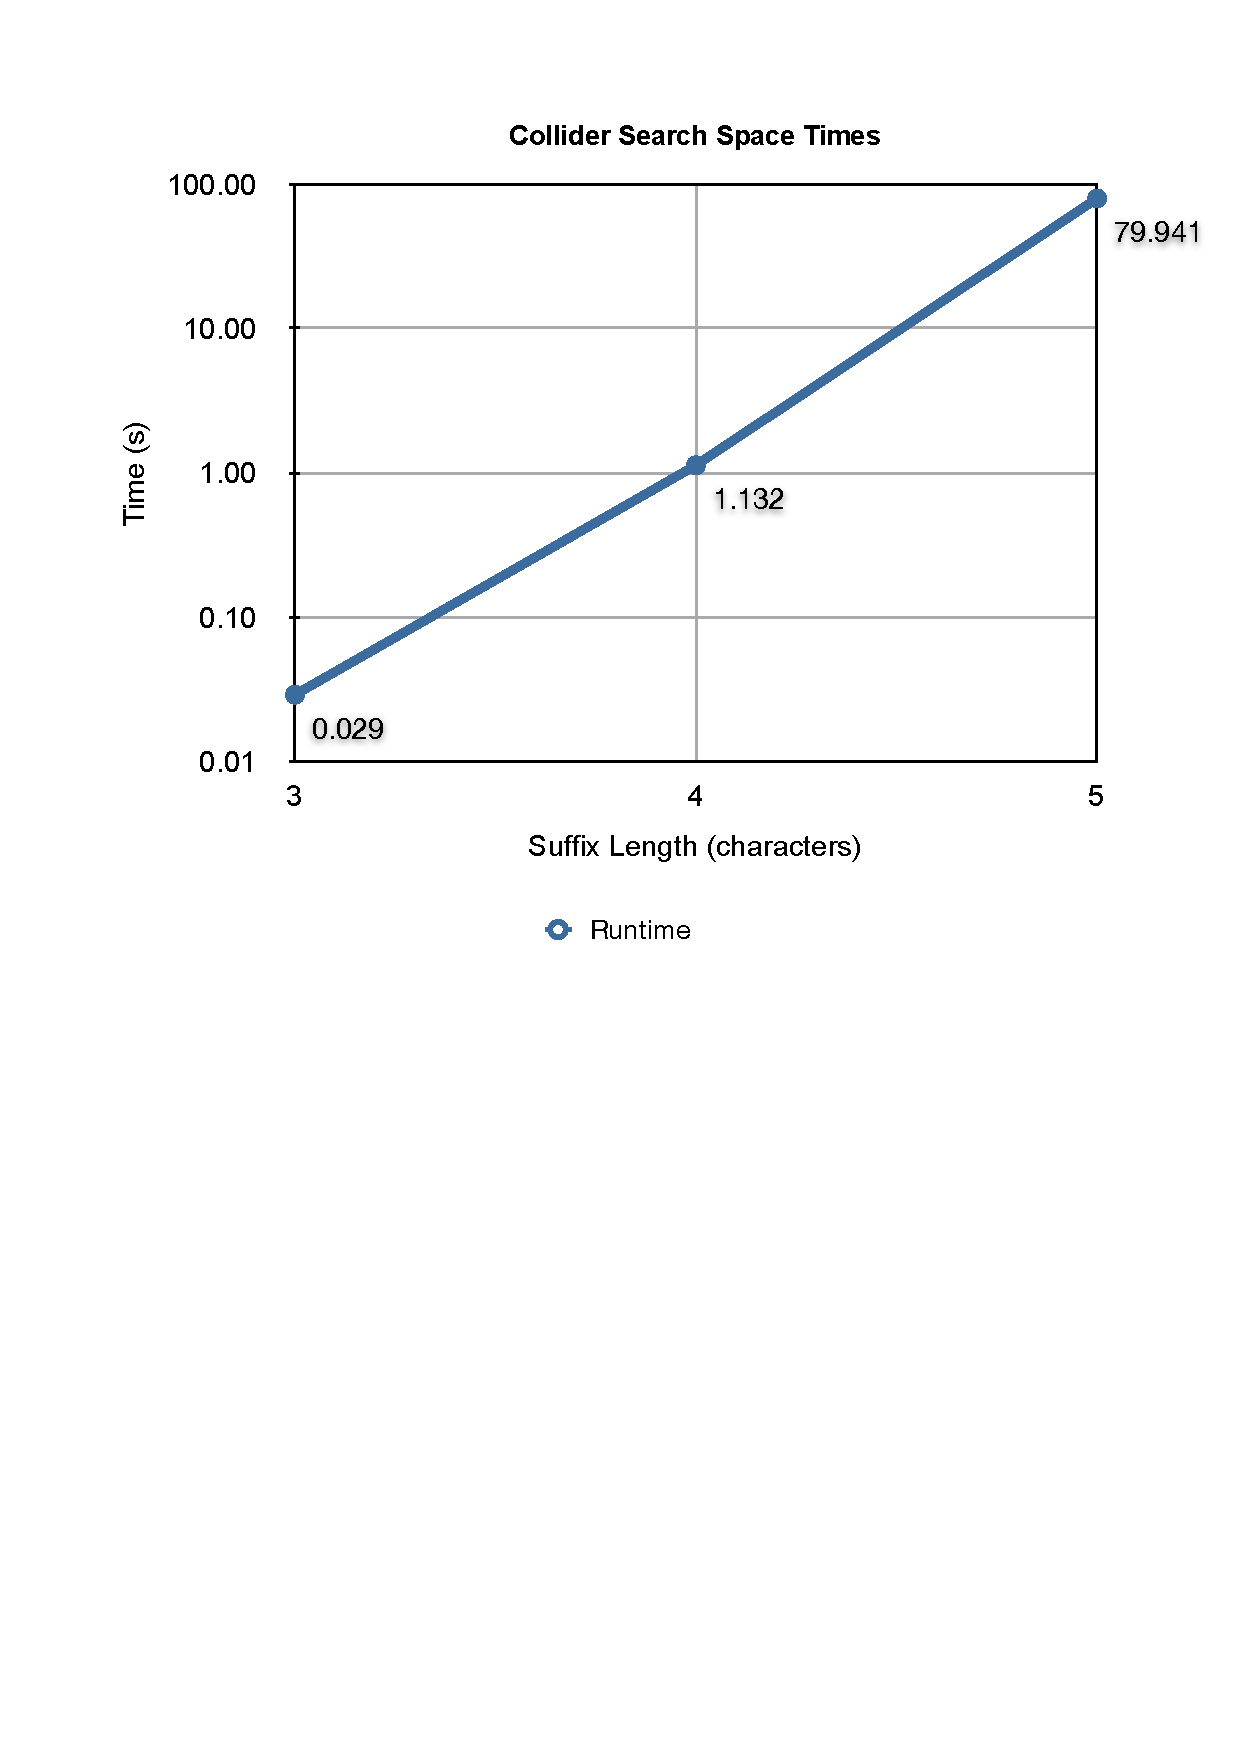
\includegraphics[scale=.5, viewport=0cm 0cm 16.6cm 13.6cm]{collider-times.pdf}
\caption{Runtime for the Collider to search the exploration spaces of sizes $62^3$, $62^4$, $62^5$ on dual quad-core Intel i5 processors.
\label{fig:collider-times}
}
\end{center}
\end{figure}

\begin{figure}
\begin{center}
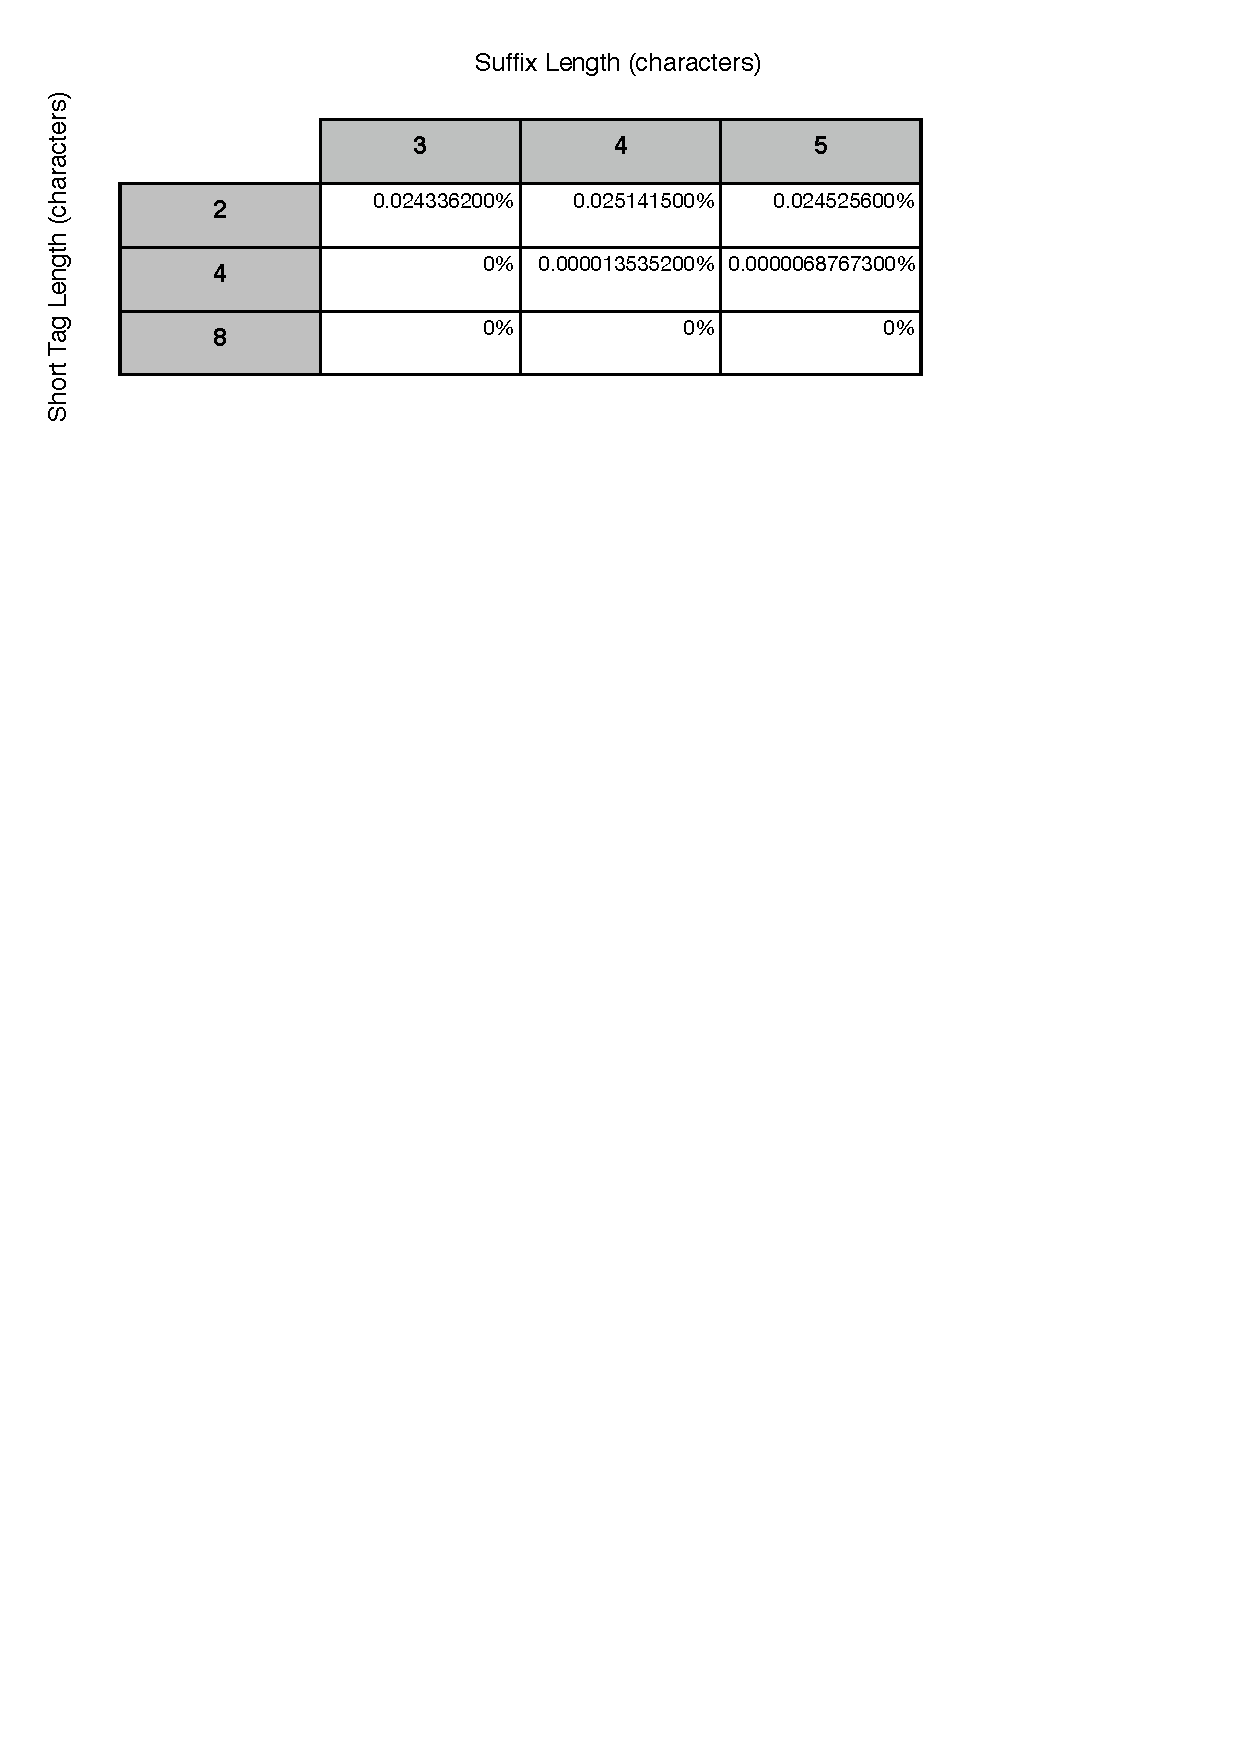
\includegraphics[scale=.5, viewport=0cm 0cm 16.5cm 7.5cm]{collider-hits.pdf}
\caption{Percent of search space that returned hits for an entered Short Tag, with a Prefix of `rice', and given Suffix Length. Length 2 prefix was `Ch', 4 was `Char', and 8 was `CharlieS'.
\label{fig:collider-hits}
}
\end{center}
\end{figure}

As expected, the runtime in Figure \ref{fig:collider-times} scales exponentially with \textit{L}, which in turn it becomes quickly infeasible for a single machine to do an exhaustive search of spaces where the suffix length is greater than 6.

Provided an attacker knows a particular group's prefix and the alphabet out of which they are generating the suffix, the embarrassingly parallel nature lends itself to brute force attacks. If we consider the adversary to be a government for example, it would be fair to assume they have thousands of machines at their disposal for such an attack. It becomes important, then for a user to pick a Plain Tag outside reasonable brute forcing bounds. 

\hl{should the `rememberable' limit discussion go here? or should this paragraph be moved out to discussion?}

Another concern is how easy it is to collide with another tag. From Fig. \ref{fig:collider-hits}, we find that beyond 4 characters, it was impossible to find collisions within easily searchable spaces (suffix sizes < 6). 

The results of these experiments place some limits on what choices a user can make currently regarding anonymity. You can only collide with up to 4 characters in a tag before the search space becomes such that any guarantee of collision is trivially small. Furthermore, $62^6$ is the upper bound on the search space for what a single computer can reasonably calculate a suffix to enable a collision with. Adding one more character to the suffix sends the computation into the span of days on a modern computer at time of writing.

However, we also show that tag collision is possible, there are certainly tunable degrees of anonymity thanks to the apparent power-log distribution of twitter tags already, and finding such a collision is feasibly done on a personal computer. \hl{What more to say here?}

\subsection{Performance}

In this experiment we wanted to see how well the encryption engine performed. In March 2011, Twitter stated that the site receives 140 million tweets per day or 1620 tweets per second on average (http://blog.twitter.com/2011/03/numbers.html). They also said that the maximum tweets per second ever was 6939. These numbers act as rough upper bounds to the number of Hoots per second the system would need to keep up with. In all likelihood, the number of encrypted messages posted would be drastically smaller than regular messages.

The benchmarks in Table \ref{tab:hps} were run on a 1.86GHz Intel Core 2 Duo, 4GB Ram, Macbook Air using Base64 encoding.


\begin{table}
\caption{Average Hoots Per Second for Encryption and Decryption
\label{tab:hps}
}
\begin{center}
    \begin{tabular}{ l  l }
	\hline
	Action & Average Hoots per second \\ \hline
	Encryption & 3614.531 \\
	Decryption & 15587.328 \\ \hline
    \end{tabular}
\end{center}
\end{table}

Given these numbers, a Twitter server could easily encrypt the entire Twitter feed as the messages were posted. To handle peak usage like the 6939 tweets per second Twitter observed, many optimizations could be made, the simplest being to add a couple computers to help with the load. Our experiment shows that the Hoot protocol does not have significant overhead during encryption or decryption, so it can be adopted with little engineering effort.

It is interesting to note that the decryption rate is important to a client, since a client will be searching tweets trying to identify and decrypt potential Hoots. A client may not trust Twitter to do the decryption since that involves sharing the Plain Tag with Twitter, so a client would decrypt the message on their machine. Almost every client will not have a datacenter of computers for decryption, but our  process can decrypt Hoots almost five times faster than it encrypts them. A client, even with limited computing power, can easily keep up with the Twitter feed.

\hl{Should experiments have a wrap up paragraph?}